% =============================================================================
%  fig_confidence.tex
%  Confidence score c vs 3rd harmonic injection I_h3
%  Data from TR-21 Study A (no-fault / healthy-line scenario)
%  Standalone compile:  pdflatex fig_confidence.tex
% =============================================================================
\documentclass[tikz, border=8pt]{standalone}
\usepackage{pgfplots}
\pgfplotsset{compat=1.18}
\usepackage{amsmath}

\begin{document}
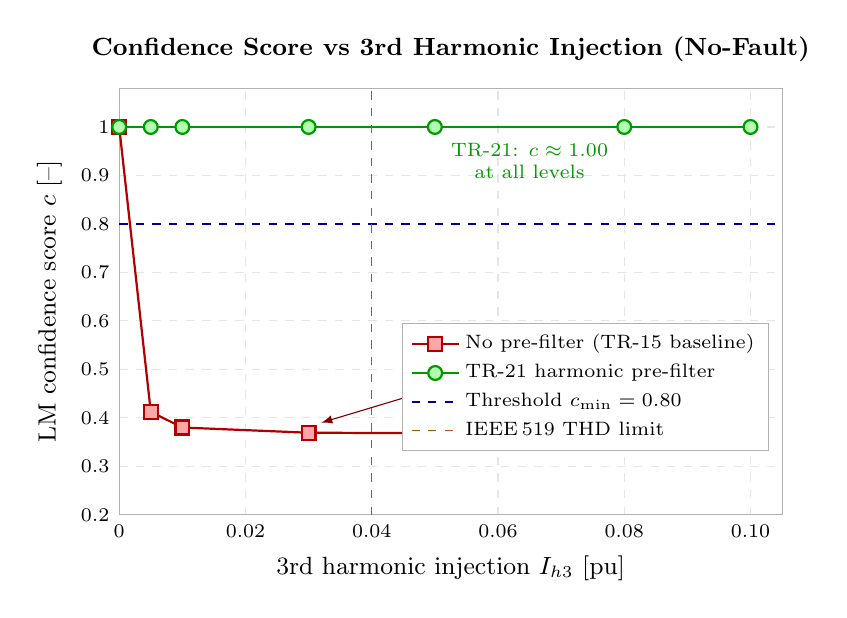
\begin{tikzpicture}
\begin{axis}[
  width         = 10cm,
  height        = 7cm,
  title         = {Confidence Score vs 3rd Harmonic Injection (No-Fault)},
  title style   = {font=\small\bfseries},
  ylabel        = {LM confidence score $c$ [--]},
  ylabel style  = {font=\small},
  xlabel        = {3rd harmonic injection $I_{h3}$ [pu]},
  xlabel style  = {font=\small},
  ymin=0.20, ymax=1.08,
  xmin=0,    xmax=0.105,
  ytick         = {0.2, 0.3, 0.4, 0.5, 0.6, 0.7, 0.8, 0.9, 1.0},
  yticklabel style = {font=\scriptsize},
  xtick         = {0, 0.02, 0.04, 0.06, 0.08, 0.10},
  xticklabels   = {0, 0.02, 0.04, 0.06, 0.08, 0.10},
  xticklabel style = {font=\scriptsize},
  legend style  = {at={(0.98, 0.45)}, anchor=north east,
                   font=\scriptsize, draw=gray!60,
                   cells={anchor=west}},
  grid          = major,
  grid style    = {gray!20, dashed},
  tick style    = {draw=none},
  axis line style = {gray!60},
  mark size     = 2.5pt,
  clip          = true,
]

% ---- No pre-filter baseline (TR-15): confidence collapses --------------------
\addplot[red!70!black, thick, mark=square*,
         mark options={fill=red!35}]
  coordinates {
    (0.000, 1.0000)
    (0.005, 0.4124)
    (0.010, 0.3801)
    (0.030, 0.3693)
    (0.050, 0.3684)
    (0.080, 0.3681)
    (0.100, 0.3680)
  };
\addlegendentry{No pre-filter (TR-15 baseline)}

% ---- TR-21 harmonic pre-filter: confidence remains at 1.0 -------------------
\addplot[green!60!black, thick, mark=*,
         mark options={fill=green!30}]
  coordinates {
    (0.000, 1.0000)
    (0.005, 1.0000)
    (0.010, 1.0000)
    (0.030, 1.0000)
    (0.050, 1.0000)
    (0.080, 1.0000)
    (0.100, 1.0000)
  };
\addlegendentry{TR-21 harmonic pre-filter}

% ---- Confidence threshold ---------------------------------------------------
\addplot[blue!60!black, thick, dashed, mark=none, domain=0:0.105, samples=2]
  ({x}, {0.80});
\addlegendentry{Threshold $c_{\min}=0.80$}

% ---- IEEE 519 THD limit (3rd harmonic dominant, THD 5% ≈ I_h3 ≈ 0.04 pu) ---
\addplot[orange!70!black, thin, dashed, mark=none]
  coordinates {(0.040, 0.20)(0.040, 1.08)};
\addlegendentry{IEEE\,519 THD limit}

% ---- Annotations ------------------------------------------------------------
\node[font=\scriptsize, red!70!black, align=center]
  at (axis cs:0.068, 0.54)
  {No filter: $c \approx 0.37$\\at any $I_{h3}>0$};
\draw[-latex, red!50!black, thin]
  (axis cs:0.055, 0.48) -- (axis cs:0.032, 0.39);

\node[font=\scriptsize, green!60!black, align=center]
  at (axis cs:0.065, 0.93)
  {TR-21: $c \approx 1.00$\\at all levels};

\end{axis}
\end{tikzpicture}
\end{document}
